\documentclass[letter,11pt]{article}

\usepackage[spanish,es-nodecimaldot]{babel}
\usepackage[utf8]{inputenc}

\usepackage{lmodern}
\usepackage[T1]{fontenc}
\usepackage{textcomp}

\usepackage{framed}
\usepackage[svgnames]{xcolor}
\colorlet{shadecolor}{Gainsboro!50}

\usepackage[labelfont=bf]{caption}
\usepackage{graphicx}
\usepackage{pstricks}

\usepackage{anysize}
\marginsize{3cm}{2cm}{2cm}{3cm}

\usepackage{siunitx}
\usepackage{amsmath}
\usepackage{array}
\usepackage{csquotes}

\usepackage{fancyhdr}
\usepackage{lastpage}
\pagestyle{fancy}
\fancyhf{}
\fancyhead[LE,RO]{Laboratorio de Circuitos Eléctricos I}
\fancyfoot[CO,CE]{\thepage\ de \pageref{LastPage}}

\special{papersize=215.9mm,279.4mm}

\usepackage[
    pdfauthor={Carlos Eduardo Caballero Burgoa},%
    pdftitle={Laboratorio de Circuitos Eléctricos I},%
    pdfsubject={La Ley de Ohm},%
    colorlinks,%
    citecolor=black,%
    filecolor=black,%
    linkcolor=black,%
    urlcolor=black,
    breaklinks]{hyperref}
\usepackage{breakurl}

\newcommand{\blankpage}{
\newpage
\thispagestyle{empty}
\mbox{}
\newpage
}

\renewcommand{\arraystretch}{1.2}

\begin{document}

\begin{titlepage}
    \begin{center}
        {\Large UNIVERSIDAD MAYOR DE SAN SIMÓN}\\
        \vspace*{0.15cm}
        {\large FACULTAD DE CIENCIAS Y TECNOLOGÍA}\\
        \vspace*{0.10cm}
        DEPARTAMENTO DE ELÉCTRICA-ELECTRÓNICA\\
        \vspace*{3.0cm}
        {\Large \textbf{LABORATORIO DE CIRCUITOS ELÉCTRICOS I}}\\
        \vspace*{0.3cm}
        {\Large \textbf{INFORME No. 1}}\\
        \vspace*{3.5cm}
        {\Large \textbf{LA LEY DE \emph{OHM}}}\\
    \end{center}

    \vspace*{6.4cm}
    \leftskip=7.95cm
    \noindent
    \textbf{Estudiante:}\\
    Caballero Burgoa, Carlos Eduardo.\\
    \newline
    \textbf{Carrera:}\\
    Ing. Electromecánica.\\
    \newline
    \textbf{Docente:}\\
    Ing. Marco Antonio Vallejo Camacho.\\
    \newline
    \textbf{Grupo:} 3E.\\
    \textbf{Fecha de entrega:} 09 de Abril del 2024.\\
\end{titlepage}

\section{Cálculos previos}

\begin{figure}[!h]
\centering
\includegraphics[scale=0.24]{resources/preinforme1.eps}
\end{figure}

\begin{figure}[!h]
\centering
\includegraphics[scale=0.24]{resources/preinforme2.eps}
\end{figure}

\section{Simulación}
Se utilizó el software \emph{Quite Universal Circuit Simulator.} para simular
el circuito, este puede verse en la figura (\ref{simulacion}).
\\

\begin{figure}[!h]
\centering
\includegraphics[scale=0.55]{resources/simulacion.eps}
\caption{Simulación de circuito.}
\label{simulacion}
\end{figure}

\newpage

\section{Tablas y mediciones}
En la figura (\ref{tablas}), se adjunta la hoja de resultados provista en la
guía de laboratorio, rellenada con la información teórica, simulada y las
mediciones realizadas en laboratorio.

\begin{figure}[!h]
\centering
\includegraphics[scale=0.22]{resources/preinforme3.eps}
\caption{Tabla de resultados.}
\label{tablas}
\end{figure}

\newpage

\section{Cuestionario}

\begin{enumerate}

\item \textbf{¿Qué cuidados hay que tener para emplear un amperímetro
digital?} \\

\begin{itemize}
    \item Asegurarse que la conexión sea correcta, teniendo en cuenta la
    polaridad y la corriente que se va a medir.
    \item Se debe apagar el circuito antes de realizar la medición.
    \item Se debe utilizar el rango apropiado para la medición de corriente, si
    se desconoce la cantidad de corriente debe usarse la escala con mayor rango.
\end{itemize}

\item \textbf{(a) Utilizando la tabla de resultados (para el voltaje $V_1$ y
corriente $I_1$) grafique la curva $I_1=V_1/R$; (b) empleando el método de
regresión lineal, calcule las constantes ``$A$'' y ``$B$'' de la ecuación
lineal, también el coeficiente de correlación ``$r^2$''; (c) ¿qué significado
tienen los valores de las constantes ``$A$'' y ``$B$'' obtenidos?; (d) ¿cuál es
el valor de la resistencia $R$ empleada?}

A partir de los datos obtenidos se genera la gráfica de la
\textbf{Figura \ref{figura}}.

\begin{figure}[!h]
\centering
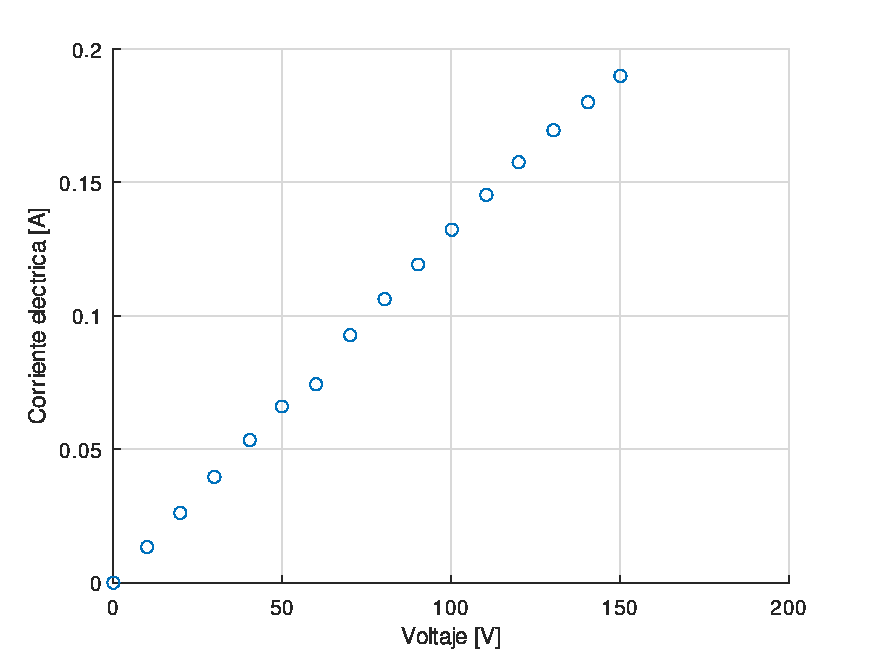
\includegraphics[width=0.85\textwidth]{resources/o1.eps}
\caption{Gráfica de voltaje vs corriente.}
\label{figura}
\end{figure}

Se calcula la recta de mejor ajuste por el método de los mínimos cuadrados, 
resultando los siguientes valores:

\begin{equation*}
    A = (\num{1.09e-3} \pm \num{1.02e-3}) [A]; 93.79\%
\end{equation*}
\begin{equation*}
    B = (\num{1.29e-3} \pm \num{1.16e-5}) [1/\Omega]; 0.90\%
\end{equation*}

Siendo su coeficiente de correlación ($r$):

\begin{equation*}
    r = 0.9994
\end{equation*}

Considerando que el modelo de ajuste es:

\begin{equation*}
    I = A + B V
\end{equation*}

$A$ representa un valor de ajuste entre las variables $I$ y $V$, y como puede
notarse es una cantidad despreciable, y puede deberse a inexactitudes en la
medición o calibración de los instrumentos.

$B$ representa la constante de proporcionalidad entre las variables $I$ y $V$, y
según la ley de \emph{Ohm} es $1/R$, conocido como la conductancia.

\begin{center}
\begin{tabular}{|>{\centering}m{9.2cm}<{\centering}|}
\hline
\textbf{Resultado}
\tabularnewline \hline
$R = (776.62 \pm \num{1.92e-11}) [\Omega]; \num{2.48e-12}\%$ \tabularnewline
\hline
\end{tabular}
\end{center}
\vspace{0.10cm}

\item \textbf{Un efecto interesante que sucede en el laboratorio, mas allá de la
diferencia que existe entre el valor medido y el indicado en las etiquetas, es
el descrito a continuación:}\\

\begin{displayquote}
    \textbf{Se realizaron mediciones en el laboratorio de las resistencias de
    valor fijo disponibles, y se encontró que durante las primeras horas de la
    mañana los valores medidos de las resistencias son unos, mientras que por
    las tardes tienen un valor mayor.}
\end{displayquote}

\textbf{¿Como puede explicar este fenómeno?}

En los materiales conductores, el aumento de la temperatura produce una
aumento en la resistencia eléctrica. Bajo la siguiente formula:

\begin{equation*}
    R_T=R_0\,(1+\alpha T)
\end{equation*}

Donde:

\begin{itemize}
    \item $R_0$: Resistencia de referencia a la temperatura $T_0$.
    \item $\alpha$: Coeficiente de temperatura, dependiente del material.
    \item $T_0$: Temperatura de referencia en la cual se conoce $R_0$.
\end{itemize}

\end{enumerate}

\section{Conclusiones}
Se demostró que la relación directamente proporcional de la ley de \emph{Ohm}
entre la corriente eléctrica y el voltaje se cumple de modo experimental.

Cuando se hace uso de los instrumentos de medición de corriente y voltaje, se
percibe que estos comienzan con valores cambiantes y después de un espacio corto
de tiempo estos se estabilizan, por tanto, es recomendable esperar un tiempo
prudencial antes de tomar la medida.

\end{document}

